\documentclass{article}
\usepackage{amsmath}
\usepackage{amssymb}
\usepackage[a4paper, margin=0.8in]{geometry}
\usepackage{graphicx}
\usepackage{algorithm}
\usepackage{algpseudocode}
\usepackage{float}
\usepackage{tikz}
\usepackage{pifont}

\setlength{\parskip}{1pt}
\setlength{\parindent}{0pt}

\newcommand{\xmark}{\ding{55}}%
\newcommand{\bioperation}{{\hspace{5pt} | \hspace{5pt}}}

\title{Asymtotic Notations}
\author{Mohammed Rizin \\ Unemployed}
\date{\today}

\begin{document}
\maketitle

\section{Types of Asymptotic Notations}

In last Section we learn the Types of Time function:
\[
\boxed{
\begin{aligned}
    1 < \log{n} < \sqrt{n} < n < n\cdot \log{n} < n^2 < n^3 < \cdots < 2^n <  3^n < n^n
\end{aligned}
}
\]

The type of Asymptotic Notations are:
\[
\begin{aligned}
    &\text{1. } O(n) &&\blacktriangleright \text{Big Oh} &&\blacktriangleright \text{Upper Bound} \\
    &\text{2. } \Omega(n) &&\blacktriangleright \text{Big Omega} &&\blacktriangleright \text{Lower Bound} \\
    &\text{3. } \Theta(n) &&\blacktriangleright \text{Theta} &&\blacktriangleright \text{Average Time Function (useful)}
\end{aligned}
\]

\subsection{Big Oh Notation}
\[
\begin{aligned}
        \text{The function } f(n) = O{(g(n))} &\leftrightarrow &\exists \text{ +ve constant $c$ and } 
        n_0 \text{ such that } f{(n)} &\leq c \cdot g{(n)} &\forall n &\geq n_0  
\end{aligned}
\]

For eg:
\[
\begin{aligned}
        f(n) &= 2n + 3 \\
        2n+3 &\leq 10n \hspace{5pt} \forall n \geq 1 \\
        f(n) &\leq 10 \cdot g(n) \\
        \text{The Time Complexity : } f(n) &= O(n)
\end{aligned}
\]

\[
\begin{aligned}
        f(n) &= 2n + 3 \\
        2n+3 &\leq 2n + 3n \\
        2n+3 &\leq 5n \hspace{5pt} \forall n \geq 1 \\
        f(n) &\leq 5 \cdot g(n) \\
        \text{Still The Time Complexity : } f(n) &= O(n)
\end{aligned}
\]

\[
\begin{aligned}
    f(n) &= 2n + 3 \\
    \text{So Can I write: }\\
        2n+3 &\leq 2n^2 + 3n^2\\ 
        2n+3 &\leq 5\cdot n^2 \hspace{5pt} \forall n \geq 1 \\
        f(n) &\leq 5 \cdot g(n) \\
        \text{Yes, Then the Time Complexity : } f(n) &= O(n^2)
\end{aligned}
\]

So I can say that $f(n) = O(n)$, $f(n) = O(n^2)$, $f(n) = O(n^3)$, $f(n) = O(2^n)$, $f(n) = O(n!)$, etc.
But we cannot say $f(n) = O(\log{n})$, $f(n) = O(\sqrt{n})$, $f(n) = O(1)$, etc.
\newline
\newline
?` Now a question arises, Why do I need to write all those if we know that $f(n) = O(n)$? 
Yeah, When we write Big Oh, we write the closest upper bound. When you any above that, it is also correct. But not usefulYeah, When we write Big Oh, we write the closest upper bound. When you any above that, it is also correct. But not useful.

\subsection{Big Omega Notation}
\[
\begin{aligned}
        \text{The function } f(n) = \Omega{(g(n))} &\leftrightarrow &\exists \text{ +ve constant $c$ and } 
        n_0 \text{ such that } f{(n)} &\geq c \cdot g{(n)} &\forall n &\geq n_0
\end{aligned}
\]

For eg:
\[
\begin{aligned}
        f(n) &= 2n + 3 \\
        2n+3 &\geq 1n \hspace{5pt} \forall n \geq 1 \\
        f(n) &\geq \underbrace{1}_c \cdot \underbrace{n}_{g(n)}\\
        \text{The Time Complexity : } f(n) &= \Omega(n)
\end{aligned}
\]

\[
\begin{aligned}
        f(n) &= 2n + 3 \\
        2n+3 &\geq 2n + 3 \\
        2n+3 &\geq 5n \hspace{5pt} \forall n \geq 1 \\
        f(n) &\geq 5 \cdot g(n) \\
        \text{Still The Time Complexity : } f(n) &= \Omega(\log{n})
\end{aligned}
\]

\[
\begin{aligned}
    f(n) &= 2n + 3 \\
    \text{So Can I write: }\\
        2n+3 &\geq 2n^2 + 3n^2\\ 
        2n+3 &\geq 5\cdot n^2 \hspace{5pt} \forall n \geq 1 \\
        f(n) &\geq 5 \cdot g(n) \\
        \text{No, the Time Complexity can't be: } f(n) &= \Omega(n^2)
\end{aligned}
\]

So which one is correct? $f(n) = \Omega(n)$ or $f(n) = \Omega(\log{n})$? Both are correct. But the closest lower bound is 
\[
\boxed{f(n) = \Omega(n)}
\]

\subsection{Theta Notation}
\[
\begin{aligned}
        \text{The function } f(n) = \Theta{(g(n))} &\leftrightarrow &\exists \text{ +ve constant $c_1$, $c_2$ and } 
        n_0 \text{ such that } c_1 \cdot g{(n)} &\leq f{(n)} \leq c_2 \cdot g{(n)} &\forall n &\geq n_0
\end{aligned}
\]

For eg:

\[
\begin{aligned}
        f(n) &= 2n + 3 \\
        1n \leq 2n &+ 3 \leq 5n  \hspace{5pt} \forall  n \geq 1 \\
        \underbrace{1}_{c1} \cdot \underbrace{n}_{g(n)} &\leq f(n) \leq \underbrace{5}_{c2} \cdot \underbrace{n}_{g(n)}\\    
\end{aligned}
\]

\[
g(n)\text{ on both sides is }n. \\
\text{So, the Time Complexity is: } \\
f(n) = \Theta(n)\\
\]


\[
\begin{aligned}
        f(n) &= 2n + 3 \\
    \underbrace{1n^2}_{\mathsf{X}}  \leq 2n &+ 3 \leq 5n^2  \hspace{5pt} \forall  n \geq 1 \\
        \text{So, the only Time Complexity : } \boxed{f(n) = \Theta(n)}\\
\end{aligned}
\]
Since I cannot find the any other $g(n)$ which satisfies the above equation, I can say that the Time Complexity is \boxed{\Theta(n)}.

\subsection{Some Myths}

People say that $f(n) = O(n)$ represent the "Worst" case. But it is not true. It is the "Upper Bound". And $f(n) = \Omega(n)$ represent the "Best" case. But it is not true. It is the "Lower Bound".
\newline
Don't get confused with the "Best" and "Worst" case with "Lower" and "Upper" bound.

\subsection{ Example 1}
\[
\begin{aligned}
    f(n) &= n! \\
    f(n) &= 1 \cdot 2 \cdot 3 \cdot 4 \cdots n \\
    1 \cdot 1 \cdot 1 \cdot 1 \cdots 1 &\leq 1 \cdot 2 \cdot 3 \cdots n \leq n \cdot n \cdot n \cdots n \hspace{5pt} \forall n \geq 1 \\
    1 &\leq n! \leq n^n \\
\end{aligned}
\]

So, we have the Upper Bound Time Complexity :  \boxed{f(n) = O(n^n)} \\
And we have the Lower Bound Time Complexity :  \boxed{f(n) = \Omega(1)} \\
There is no $g(n)$ which satisfies the above equation. So, the Average Time Complexity doesn't exist.


The best Asymptotic Notation is $\Theta(n)$. Because it gives the average time function. It is useful.
Suppose you are buying a mobile phone and the shopkeeper says that there are phones between 2000 and 200000 even though you said that you want a phone for 20000. 2000 is the lower bound and 200000 is the upper bound. Are they wrong
? No. But it is not useful. So, the best Asymptotic Notation is $\Theta(n)$. 
If you are telling me the Big Oh , i don't know whether it is nearest upper bound or not. So, it is not useful. So, the best Asymptotic Notation is $\Theta(n)$.
Big Oh and Big Omega are mainly useful in case of $n!$.

\begin{enumerate}
    \item The function $f(n)$ belong to the $n$ class. So everything above it is upper bound. So the upper bound of $f(n)$ could be $O(n)$, $O(n^2)$, $O(n^3)$, $O(2^n)$, $O(n!)$, etc.

    \item The function $f(n)$ belong to the $n$ class. So everything below it is lower bound. So the lower bound of $f(n)$ could be $\Omega(n)$, $\Omega(\sqrt{n})$, $\Omega(\log{n})$, $\Omega(1)$, etc.

    \item The function $f(n)$ belong to the $n$ class. So everything equal to it is average bound. So the average bound of $f(n)$ could be $\Theta(n)$.
\end{enumerate}

\section{Properties of Asymptotic Notations}

\subsection{General Properties}
\begin{enumerate}
\item if $f(n)$ is $O(g(n))$  then $a* f(n)$ is $O(g(n))$ for any constant $a > 0$.\\
eg: $f(n) = 2n^2 + 3$ is $O(n^2)$\\
then $2f(n) = 4n^2 + 6$ is $O(n^2)$\\
This is true for all three Asymptotic Notations.

\item Reflexive Property: if $f(n)$ is given then $f(n)$ is $O(f(n))$\\
eg : $f(n) = n^2$ is $O(n^2)$\\
This is true for all three Asymptotic Notations.\\
\item Transitive Property: if $f(n)$ is $O(g(n))$ and $g(n)$ is $O(h(n))$ then $f(n)$ is $O(h(n))$\\
eg: $f(n) = n^2$ is $O(n^3)$ and $n^3$ is $O(n^4)$ then $f(n)$ is $O(n^4)$\\
This is true for all three Asymptotic Notations.\\
\item Symmetric Property: if $f(n)$ is $\Theta(g(n))$ then $g(n)$ is $\Theta(f(n))$\\
eg: $f(n) = n^2$ is $\Theta(n^2)$ then $n^2$ is $\Theta(n^2)
$\\
This is true for only $\Theta$ Asymptotic Notation.\\
\item Transpose Symmetric: if $f(n)$ is $O(g(n))$ then $g(n)$ is $\Omega(f(n))$\\
eg: $f(n) = n^2$ is $O(n^3)$ then $n^3$ is $\Omega(n^2)$\\
This is true for both $O \text{ and }\Omega$ Notations.\\

\item if $f(n) = O(g(n))$ and $f(n) = \Omega(g(n))$ then 



\[
\centering
\begin{aligned}
    \overbrace{g(n)}^{\downarrow} \leq f(n) \leq \overbrace{g(n)}^{\downarrow} \\
    \boxed{f(n) = \Theta(g(n))}\\
\end{aligned}
\]

\item if $f(n) = O(g(n))$ and $d(n) = O(e(n))$ then $f(n) \pm d(n) = O(max(g(n), e(n)))$\\
eg: \\
\quad $f(n) = n^2$ is $O(n^2)$ \\ \quad and $d(n) = n^3$ is $O(n^3)$ \\ \quad then $f(n) \pm d(n) = n^2 + n^3 is O(n^3)$\\

\item if $f(n) = O(g(n))$ and $d(n) = O(e(n))$ then $f(n) \cdot d(n) = O(g(n) \cdot e(n))$\\
eg: \\
\quad $f(n) = n^2$ is $O(n^2)$ \\ \quad and $d(n) = n^3$ is $O(n^3)$ \\ \quad then $f(n) \cdot d(n) = n^2 \cdot n^3 is O(n^5)$\\
\end{enumerate}

\section{Comparison of functions}

For eg : Between $n^2$ and $n^3$ which one is greater?
1. Method 1: Sample Method
\[
\begin{aligned}
    n = 1 &\rightarrow 1^2 = 1 \hspace{5pt} \text{and} \hspace{5pt} 1^3 = 1 \\
    n = 2 &\rightarrow 2^2 = 4 \hspace{5pt} \text{and} \hspace{5pt} 2^3 = 8 \\
    n = 3 &\rightarrow 3^2 = 9 \hspace{5pt} \text{and} \hspace{5pt} 3^3 = 27 \\
    n = 4 &\rightarrow 4^2 = 16 \hspace{5pt} \text{and} \hspace{5pt} 4^3 = 64 \\
    n = 5 &\rightarrow 5^2 = 25 \hspace{5pt} \text{and} \hspace{5pt} 5^3 = 125 \\
\end{aligned}
\]  
So, $n^3$ is greater than $n^2$.

2. Method 2: Apply Log on both sides
\[
\begin{aligned}
    n^2 &\leq n^3 \\
    \log{n^2} &\leq \log{n^3} \\
    2\log{n} &\leq 3\log{n} \\
    2 &\leq 3 \\
\end{aligned}
\]  
So, $n^3$ is greater than $n^2$.

\textbf{Logarithm Properties: } \\
\[ 
\begin{aligned}
    \log{ab} &= \log{a} + \log{b} \\
    \log{\frac{a}{b}} &= \log{a} - \log{b} \\
    \log{a^b} &= b\log{a} \\
    a^{\log_c{b}} &= b^{\log_c{a}} \\
    a^b = n &\rightarrow b = \log_a{n} \\
\end{aligned}
\]

For Example: \\
Which is greater $n^2\log{n} \text{ or } n{(\log{n})}^{10}$? \\
\[
\begin{aligned}
    n^2\log{n} &\bioperation n{(\log{n})}^{10} \\
    2\log{n} + \log(\log{n}) &\bioperation \log{n} + 10{\log(\log{n})} \\
    \text{Bigger term is $\log{n}$ and } &\log({\log{n}}) \text{ becomes negligible}\\
    2\log{n} &\geq \log{n} \\
\end{aligned}
\]
So, $n^2\log{n}$ is greater than $n{(\log{n})}^{10}$.

\[
\begin{aligned}
    \text{Which is greater } f(n) = 3n^{\sqrt{n}} &\text{ or } 2^{\sqrt{n}\cdot \log_2{n}}? \\
    3n^{\sqrt{n}} &\bioperation 2^{\sqrt{n}\cdot \log_2{n}} \\
    3n^{\sqrt{n}} &\bioperation 2^{\log_2{n^{\sqrt{n}}}} \\
    3n^{\sqrt{n}} &\bioperation {n^{\sqrt{n}}}^{\log_2{2} = 1} \\
    3n^{\sqrt{n}} &\simeq  n^{\sqrt{n}} \\
    \text{ Asymtotically both} &\text{ are equal.} \\
\end{aligned}
\]

\[
\begin{aligned}
    \text{Which is greater } f(n) = 2^n &\text{ or } 2^{2n}? \\
    2^n &\bioperation 2^{2n} \\
    \text{Applying }\log &\text{ on both sides, }\\
    n &< 2n \\
    \text{ Asymtotically we cannot say both} &\text{ are equal after applying } \log \\
\end{aligned}
\]

\textbf{Another Example:} \\ 
\[ 
\begin{aligned}
f_1(n) &=     
\begin{cases} 
      n^3 & n < 100 \\
      n^2 & n \geq 100\\
\end{cases}\\
f_2(n) &=     
\begin{cases} 
      n^2 & n < 10000 \\
      n^2 & n \geq 10000\\
\end{cases}\\
\\
\text{Which is greater } f_1(n) &\text{ or } f_2(n)? \\
\end{aligned}
\]
%draw a number line just draw
\begin{center}
    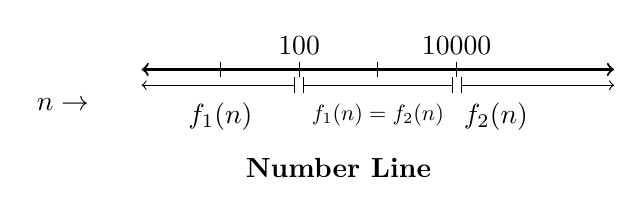
\begin{tikzpicture}
        % Draw the number line
        \draw[thick,<->] (0,0) -- (6,0) ;
        \node[below] at (2.5,-1.0 ) {\textbf{Number Line}};
        \node[below] at (-1.0,-0.25) {$n \rightarrow$};
        
        \foreach \x/\label in {1/100, 2/100, 3/1000, 4/10000} {
            \draw (\x,0.1) -- (\x,-0.1);
            \ifnum\x=2
                \node at (\x,0.3) {\label};
            \fi
            \ifnum\x=4 
                \node at (\x,0.3) {\label};
            \fi
        }
        \draw[thin,<-|] (0,-0.2) -- (1.95,-0.2);
        \node[below] at (1,-0.3) {$f_1(n)$};

        \draw[thin,|-|] (2.05,-0.2) -- (3.95,-0.2);
        \node[below, scale=0.8] at (3,-0.34) {$f_1(n) = f_2(n)$};

        \draw[thin,|->] (4.05,-0.2) -- (6,-0.2);
        \node[below] at (4.5,-0.3) {$f_2(n)$};
    \end{tikzpicture}
\end{center}
\begin{center}
Since $f_2(n)$ is greater than $f_1(n)$ $ \forall n \geq 10000$. So, $f_2(n)$ is greater than $f_1(n)$.
\end{center}

\end{document}